\documentclass[]{article}
\usepackage{lmodern}
\usepackage{amssymb,amsmath}
\usepackage{ifxetex,ifluatex}
\usepackage{fixltx2e} % provides \textsubscript
\ifnum 0\ifxetex 1\fi\ifluatex 1\fi=0 % if pdftex
  \usepackage[T1]{fontenc}
  \usepackage[utf8]{inputenc}
\else % if luatex or xelatex
  \ifxetex
    \usepackage{mathspec}
  \else
    \usepackage{fontspec}
  \fi
  \defaultfontfeatures{Ligatures=TeX,Scale=MatchLowercase}
\fi
% use upquote if available, for straight quotes in verbatim environments
\IfFileExists{upquote.sty}{\usepackage{upquote}}{}
% use microtype if available
\IfFileExists{microtype.sty}{%
\usepackage{microtype}
\UseMicrotypeSet[protrusion]{basicmath} % disable protrusion for tt fonts
}{}
\usepackage[margin=1in]{geometry}
\usepackage{hyperref}
\hypersetup{unicode=true,
            pdftitle={Lab Three: Visualizing Data, Probability, the Normal Distribution, and Z Scores},
            pdfauthor={Alex Davis; Cody Adams},
            pdfborder={0 0 0},
            breaklinks=true}
\urlstyle{same}  % don't use monospace font for urls
\usepackage{color}
\usepackage{fancyvrb}
\newcommand{\VerbBar}{|}
\newcommand{\VERB}{\Verb[commandchars=\\\{\}]}
\DefineVerbatimEnvironment{Highlighting}{Verbatim}{commandchars=\\\{\}}
% Add ',fontsize=\small' for more characters per line
\usepackage{framed}
\definecolor{shadecolor}{RGB}{248,248,248}
\newenvironment{Shaded}{\begin{snugshade}}{\end{snugshade}}
\newcommand{\KeywordTok}[1]{\textcolor[rgb]{0.13,0.29,0.53}{\textbf{#1}}}
\newcommand{\DataTypeTok}[1]{\textcolor[rgb]{0.13,0.29,0.53}{#1}}
\newcommand{\DecValTok}[1]{\textcolor[rgb]{0.00,0.00,0.81}{#1}}
\newcommand{\BaseNTok}[1]{\textcolor[rgb]{0.00,0.00,0.81}{#1}}
\newcommand{\FloatTok}[1]{\textcolor[rgb]{0.00,0.00,0.81}{#1}}
\newcommand{\ConstantTok}[1]{\textcolor[rgb]{0.00,0.00,0.00}{#1}}
\newcommand{\CharTok}[1]{\textcolor[rgb]{0.31,0.60,0.02}{#1}}
\newcommand{\SpecialCharTok}[1]{\textcolor[rgb]{0.00,0.00,0.00}{#1}}
\newcommand{\StringTok}[1]{\textcolor[rgb]{0.31,0.60,0.02}{#1}}
\newcommand{\VerbatimStringTok}[1]{\textcolor[rgb]{0.31,0.60,0.02}{#1}}
\newcommand{\SpecialStringTok}[1]{\textcolor[rgb]{0.31,0.60,0.02}{#1}}
\newcommand{\ImportTok}[1]{#1}
\newcommand{\CommentTok}[1]{\textcolor[rgb]{0.56,0.35,0.01}{\textit{#1}}}
\newcommand{\DocumentationTok}[1]{\textcolor[rgb]{0.56,0.35,0.01}{\textbf{\textit{#1}}}}
\newcommand{\AnnotationTok}[1]{\textcolor[rgb]{0.56,0.35,0.01}{\textbf{\textit{#1}}}}
\newcommand{\CommentVarTok}[1]{\textcolor[rgb]{0.56,0.35,0.01}{\textbf{\textit{#1}}}}
\newcommand{\OtherTok}[1]{\textcolor[rgb]{0.56,0.35,0.01}{#1}}
\newcommand{\FunctionTok}[1]{\textcolor[rgb]{0.00,0.00,0.00}{#1}}
\newcommand{\VariableTok}[1]{\textcolor[rgb]{0.00,0.00,0.00}{#1}}
\newcommand{\ControlFlowTok}[1]{\textcolor[rgb]{0.13,0.29,0.53}{\textbf{#1}}}
\newcommand{\OperatorTok}[1]{\textcolor[rgb]{0.81,0.36,0.00}{\textbf{#1}}}
\newcommand{\BuiltInTok}[1]{#1}
\newcommand{\ExtensionTok}[1]{#1}
\newcommand{\PreprocessorTok}[1]{\textcolor[rgb]{0.56,0.35,0.01}{\textit{#1}}}
\newcommand{\AttributeTok}[1]{\textcolor[rgb]{0.77,0.63,0.00}{#1}}
\newcommand{\RegionMarkerTok}[1]{#1}
\newcommand{\InformationTok}[1]{\textcolor[rgb]{0.56,0.35,0.01}{\textbf{\textit{#1}}}}
\newcommand{\WarningTok}[1]{\textcolor[rgb]{0.56,0.35,0.01}{\textbf{\textit{#1}}}}
\newcommand{\AlertTok}[1]{\textcolor[rgb]{0.94,0.16,0.16}{#1}}
\newcommand{\ErrorTok}[1]{\textcolor[rgb]{0.64,0.00,0.00}{\textbf{#1}}}
\newcommand{\NormalTok}[1]{#1}
\usepackage{graphicx,grffile}
\makeatletter
\def\maxwidth{\ifdim\Gin@nat@width>\linewidth\linewidth\else\Gin@nat@width\fi}
\def\maxheight{\ifdim\Gin@nat@height>\textheight\textheight\else\Gin@nat@height\fi}
\makeatother
% Scale images if necessary, so that they will not overflow the page
% margins by default, and it is still possible to overwrite the defaults
% using explicit options in \includegraphics[width, height, ...]{}
\setkeys{Gin}{width=\maxwidth,height=\maxheight,keepaspectratio}
\IfFileExists{parskip.sty}{%
\usepackage{parskip}
}{% else
\setlength{\parindent}{0pt}
\setlength{\parskip}{6pt plus 2pt minus 1pt}
}
\setlength{\emergencystretch}{3em}  % prevent overfull lines
\providecommand{\tightlist}{%
  \setlength{\itemsep}{0pt}\setlength{\parskip}{0pt}}
\setcounter{secnumdepth}{0}
% Redefines (sub)paragraphs to behave more like sections
\ifx\paragraph\undefined\else
\let\oldparagraph\paragraph
\renewcommand{\paragraph}[1]{\oldparagraph{#1}\mbox{}}
\fi
\ifx\subparagraph\undefined\else
\let\oldsubparagraph\subparagraph
\renewcommand{\subparagraph}[1]{\oldsubparagraph{#1}\mbox{}}
\fi

%%% Use protect on footnotes to avoid problems with footnotes in titles
\let\rmarkdownfootnote\footnote%
\def\footnote{\protect\rmarkdownfootnote}

%%% Change title format to be more compact
\usepackage{titling}

% Create subtitle command for use in maketitle
\newcommand{\subtitle}[1]{
  \posttitle{
    \begin{center}\large#1\end{center}
    }
}

\setlength{\droptitle}{-2em}

  \title{Lab Three: Visualizing Data, Probability, the Normal Distribution, and Z
Scores}
    \pretitle{\vspace{\droptitle}\centering\huge}
  \posttitle{\par}
    \author{Alex Davis \\ Cody Adams}
    \preauthor{\centering\large\emph}
  \postauthor{\par}
    \date{}
    \predate{}\postdate{}
  

\begin{document}
\maketitle

This lab discusses the basics of visualizing data, probability, the
normal distribution, and z scores. The following packages are required
for this lab:

\begin{enumerate}
\def\labelenumi{\arabic{enumi}.}
\tightlist
\item
  sfsmisc
\item
  psych
\item
  car
\item
  tidyverse
\end{enumerate}

\subsection{Part I: Histograms and
Density}\label{part-i-histograms-and-density}

Recall that histograms are used to visualize continuous data. Histograms
are not used to visualize categorical data. Instead, a bar plot is
advised for categorical data. The \texttt{geom\_hist()} function creates
histograms in R using ggplot visualizations. The following is an example
of creating a histogram of the \texttt{age} variable within the
\texttt{ds} data set.

\begin{Shaded}
\begin{Highlighting}[]
\KeywordTok{ggplot}\NormalTok{(ds, }\KeywordTok{aes}\NormalTok{(age)) }\OperatorTok{+}
\StringTok{  }\KeywordTok{geom_histogram}\NormalTok{()}
\end{Highlighting}
\end{Shaded}

\begin{verbatim}
## `stat_bin()` using `bins = 30`. Pick better value with `binwidth`.
\end{verbatim}

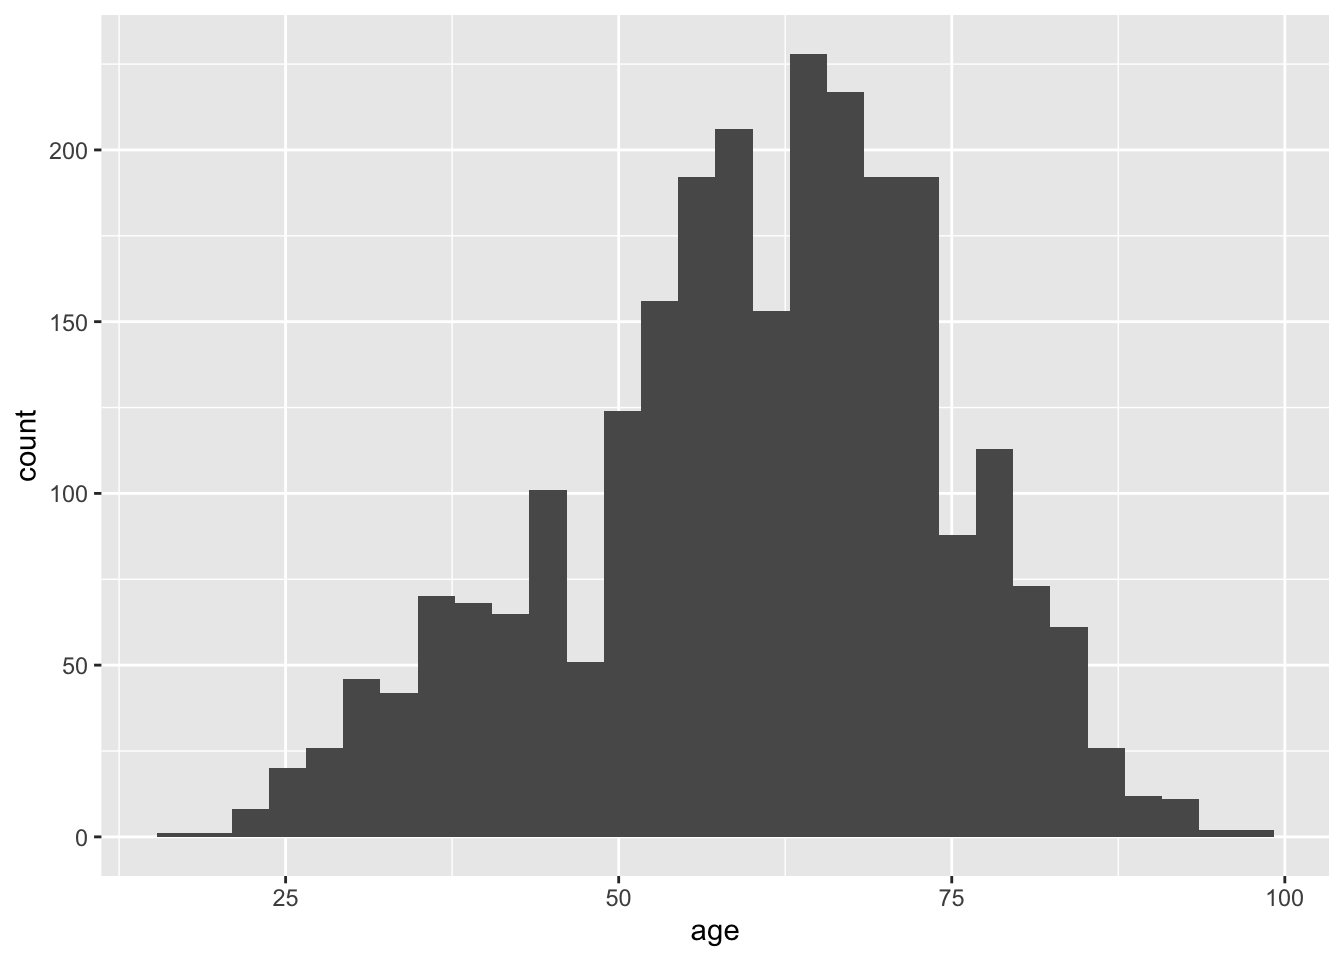
\includegraphics{lab3_files/figure-latex/3_hist1-1.pdf}

The histogram displays the frequency of \texttt{age} for given bins.
Alternatively, the density of \texttt{age} can be shown instead of
frequency by making a slight change in the visualization. Use the
mapping aesthetic inside the \texttt{geom\_histogram()} function and
setting x as the age variable and y as \texttt{..density..}

\begin{Shaded}
\begin{Highlighting}[]
\KeywordTok{ggplot}\NormalTok{(ds) }\OperatorTok{+}
\StringTok{  }\KeywordTok{geom_histogram}\NormalTok{(}\KeywordTok{aes}\NormalTok{(}\DataTypeTok{x=}\NormalTok{age, }\DataTypeTok{y=}\NormalTok{..density..))}
\end{Highlighting}
\end{Shaded}

\begin{verbatim}
## `stat_bin()` using `bins = 30`. Pick better value with `binwidth`.
\end{verbatim}

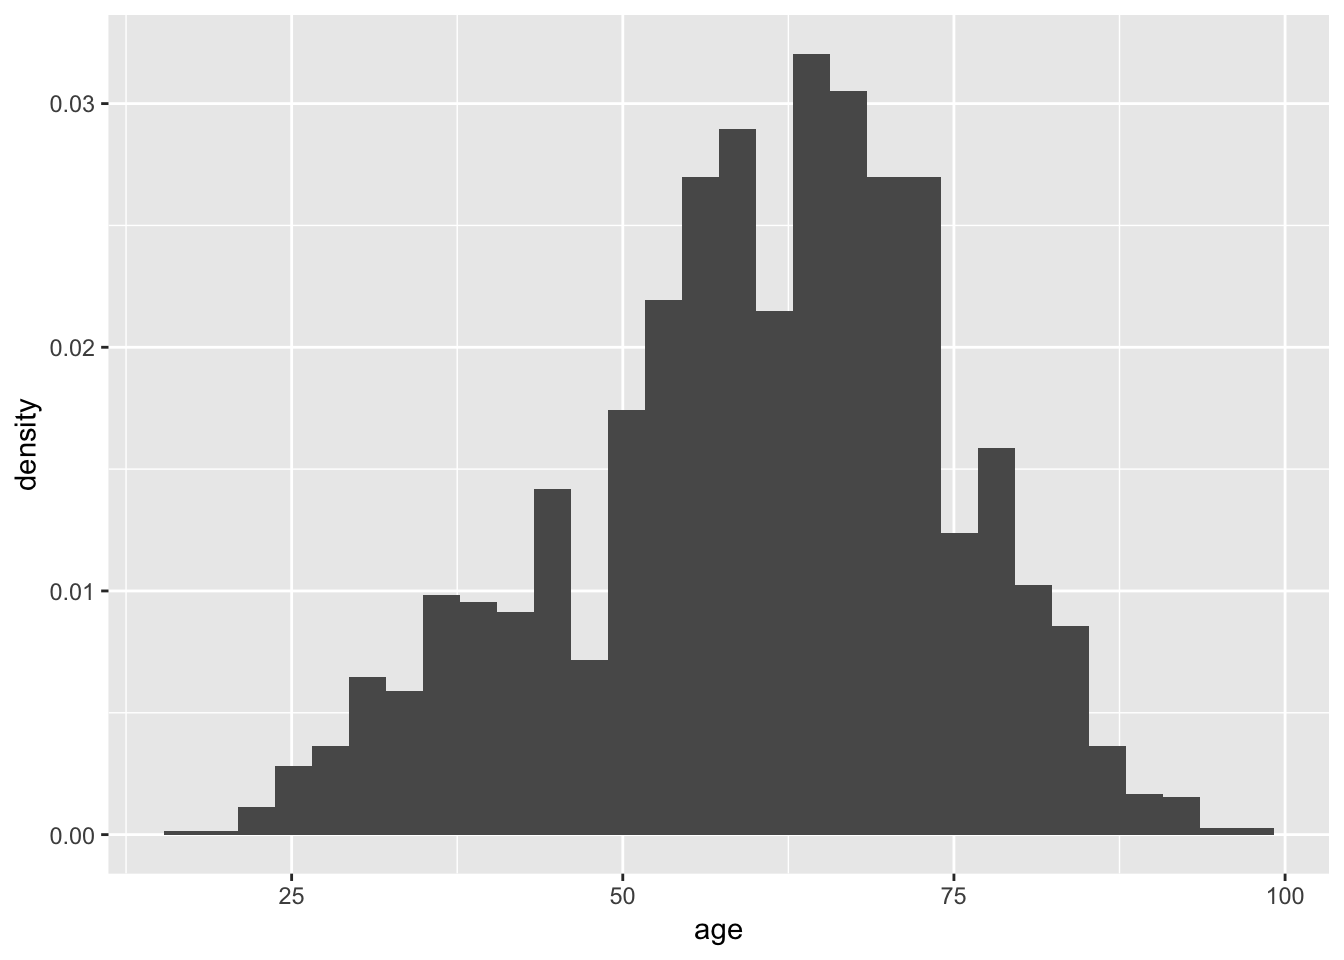
\includegraphics{lab3_files/figure-latex/3_hist2-1.pdf}

The shape of the plot is the same for the frequency and density
histograms; however, the y-axis measures in different units. The area
associated with the largest y-axis value suggest that a higher
percentage of respondents are likely to provide an age within the ages
on the x-axis.

Data is organized into ranges, known as bins, to compose the x-axis. The
number of bins is a potentially contentious topic; however, a good
recommendation is to set the number of bins equal to \(\sqrt n\), where
n is the number of observations. To change the number of bins, use
\texttt{bins=n} inside the \texttt{geom\_histogram()} function. The
square root of n for the current data set is a little over 50, so set
the bins to be 50.

\begin{Shaded}
\begin{Highlighting}[]
\KeywordTok{ggplot}\NormalTok{(ds, }\KeywordTok{aes}\NormalTok{(age)) }\OperatorTok{+}
\StringTok{  }\KeywordTok{geom_histogram}\NormalTok{(}\DataTypeTok{bins=}\DecValTok{50}\NormalTok{)}
\end{Highlighting}
\end{Shaded}

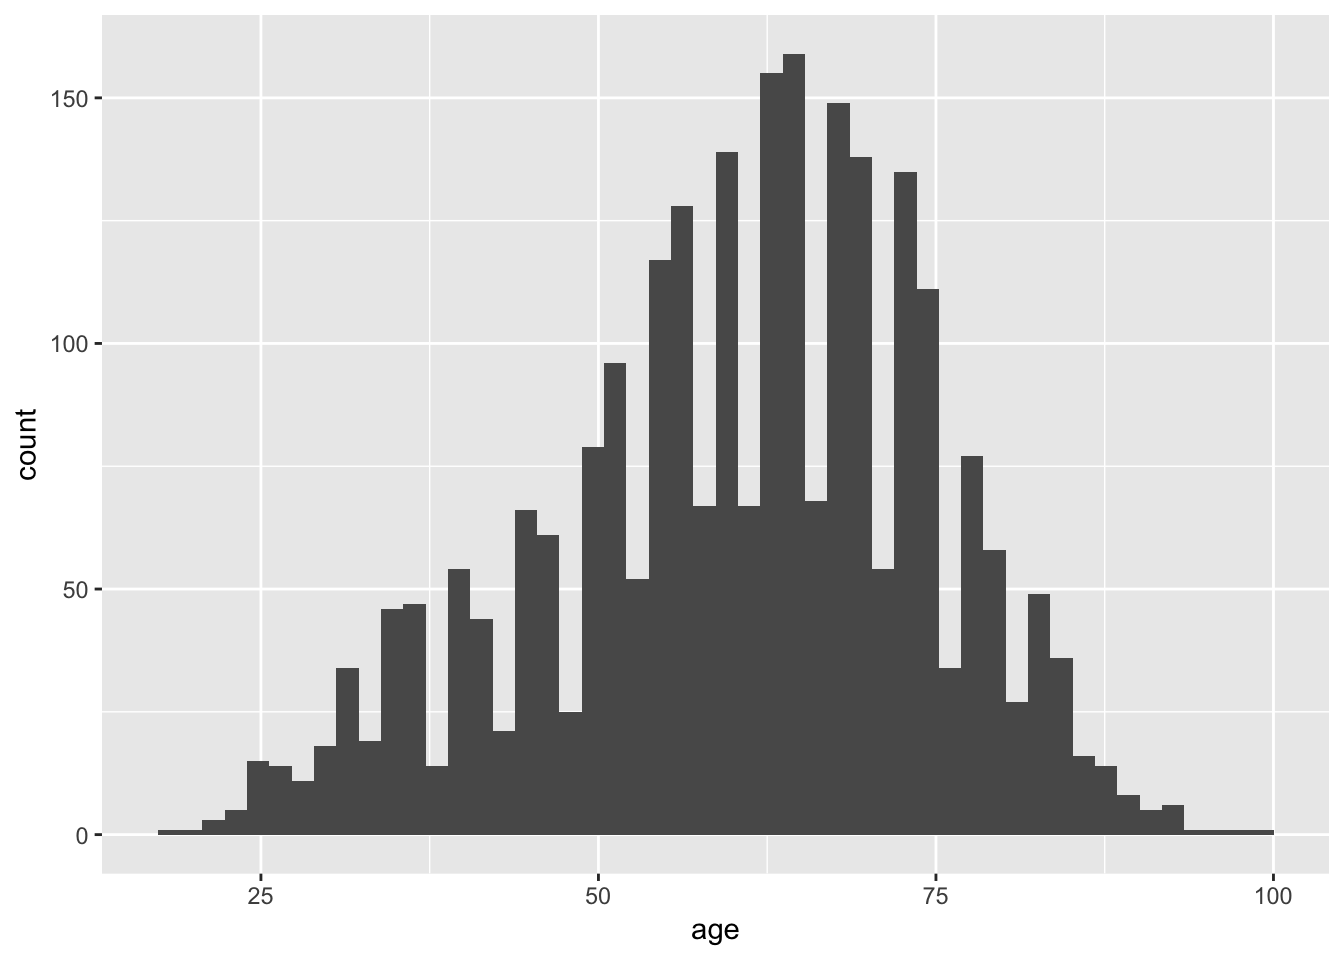
\includegraphics{lab3_files/figure-latex/3_hist3-1.pdf}

Using various functions along with the histogram function, the
visualization is improved with more meaningful information. These
functions can help:

\begin{enumerate}
\def\labelenumi{\arabic{enumi}.}
\tightlist
\item
  xlab(``X-Axis Label'')

  \begin{itemize}
  \tightlist
  \item
    Sets the label for the x-axis
  \end{itemize}
\item
  ylab(``Y-Axis label'')

  \begin{itemize}
  \tightlist
  \item
    Sets the label for the y-axis
  \end{itemize}
\item
  ggtitle(``Title'')

  \begin{itemize}
  \tightlist
  \item
    Sets the histogram title
  \end{itemize}
\item
  coord\_cartesian(ylim=c(min:max), xlim=c(min:max))

  \begin{itemize}
  \tightlist
  \item
    Sets the limits of the x and y axes.
  \end{itemize}
\end{enumerate}

The following is an excellent example of a histogram of the \texttt{age}
data.

\begin{Shaded}
\begin{Highlighting}[]
\KeywordTok{ggplot}\NormalTok{(ds, }\KeywordTok{aes}\NormalTok{(age)) }\OperatorTok{+}
\StringTok{  }\KeywordTok{geom_histogram}\NormalTok{(}\DataTypeTok{bins=}\DecValTok{50}\NormalTok{) }\OperatorTok{+}\StringTok{ }
\StringTok{  }\KeywordTok{xlab}\NormalTok{(}\StringTok{"Age"}\NormalTok{) }\OperatorTok{+}
\StringTok{  }\KeywordTok{ylab}\NormalTok{(}\StringTok{"Frequency"}\NormalTok{) }\OperatorTok{+}
\StringTok{  }\KeywordTok{ggtitle}\NormalTok{(}\StringTok{"Histogram of Age"}\NormalTok{) }\OperatorTok{+}
\StringTok{  }\KeywordTok{coord_cartesian}\NormalTok{(}\DataTypeTok{ylim=}\KeywordTok{c}\NormalTok{(}\DecValTok{0}\NormalTok{,}\DecValTok{175}\NormalTok{), }\DataTypeTok{xlim=}\KeywordTok{c}\NormalTok{(}\DecValTok{15}\NormalTok{,}\DecValTok{95}\NormalTok{)) }\OperatorTok{+}
\StringTok{  }\KeywordTok{theme_light}\NormalTok{() }\CommentTok{# Sets the theme. There are a lot to choose from.}
\end{Highlighting}
\end{Shaded}

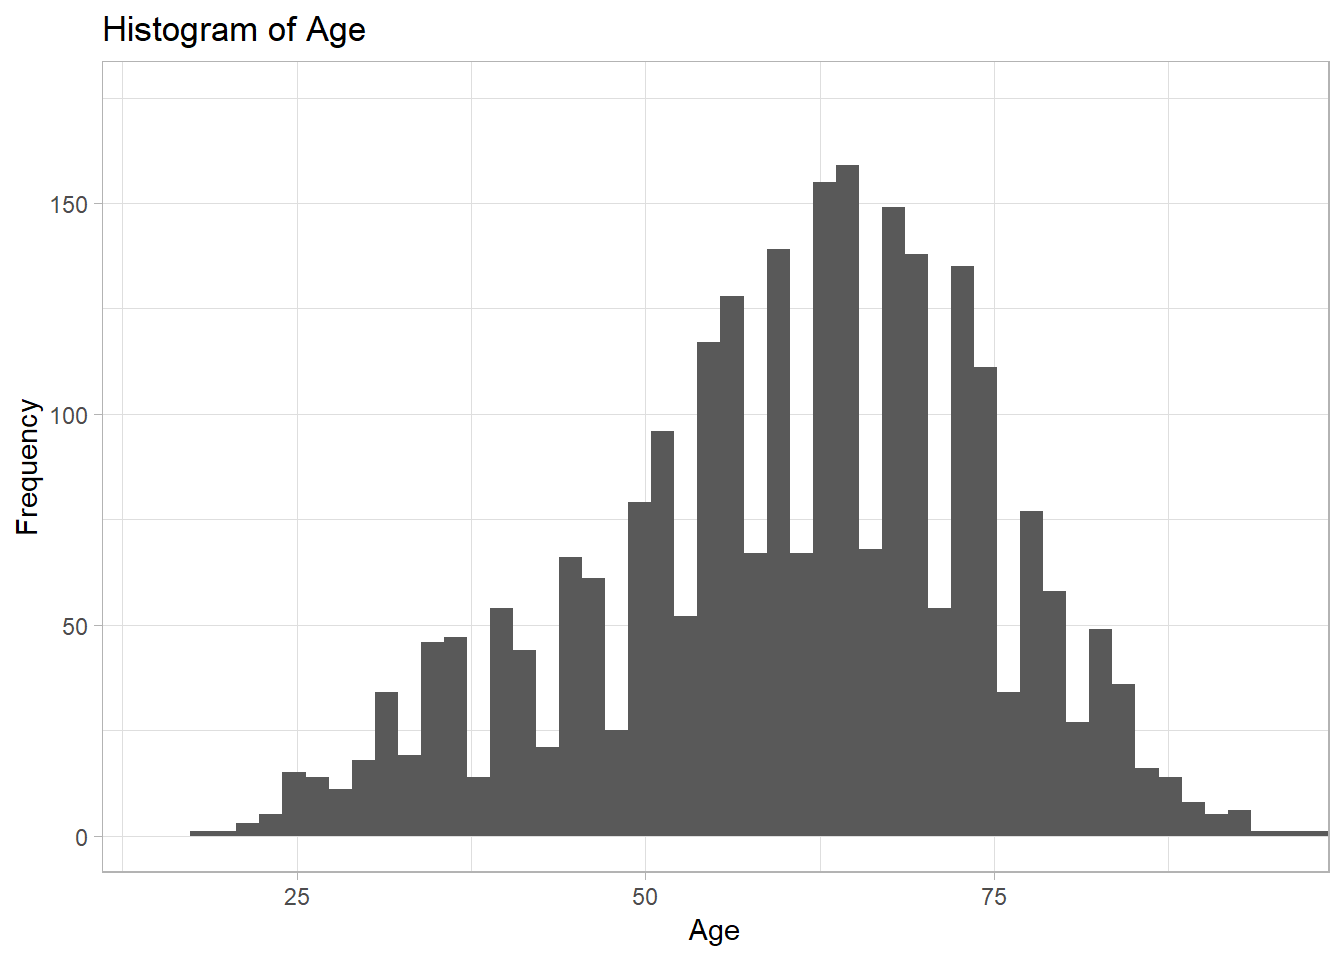
\includegraphics{lab3_files/figure-latex/3_hist5-1.pdf}

\subsubsection{Normal Distribution and
Histograms}\label{normal-distribution-and-histograms}

Data approximated by the normal distribution can define probabilities.
Using R, the normal distribution ``bell curve'' can be projected over a
histogram.

Given an identified mean and standard deviation, and a density
histogram, the \texttt{stat\_function()} function can project a normal
distribution as follows. Specify \texttt{fun=dnorm}.

\begin{Shaded}
\begin{Highlighting}[]
\KeywordTok{ggplot}\NormalTok{(ds, }\KeywordTok{aes}\NormalTok{(age)) }\OperatorTok{+}
\StringTok{  }\KeywordTok{geom_histogram}\NormalTok{(}\KeywordTok{aes}\NormalTok{(}\DataTypeTok{x=}\NormalTok{age, }\DataTypeTok{y=}\NormalTok{..density..), }\DataTypeTok{bins=}\DecValTok{50}\NormalTok{) }\OperatorTok{+}
\StringTok{  }\KeywordTok{stat_function}\NormalTok{(}\DataTypeTok{fun=}\NormalTok{dnorm, }\DataTypeTok{args =} \KeywordTok{list}\NormalTok{(}\DataTypeTok{mean=}\KeywordTok{mean}\NormalTok{(ds}\OperatorTok{$}\NormalTok{age), }\DataTypeTok{sd=}\KeywordTok{sd}\NormalTok{(ds}\OperatorTok{$}\NormalTok{age)), }\DataTypeTok{color=}\StringTok{"red"}\NormalTok{)}
\end{Highlighting}
\end{Shaded}

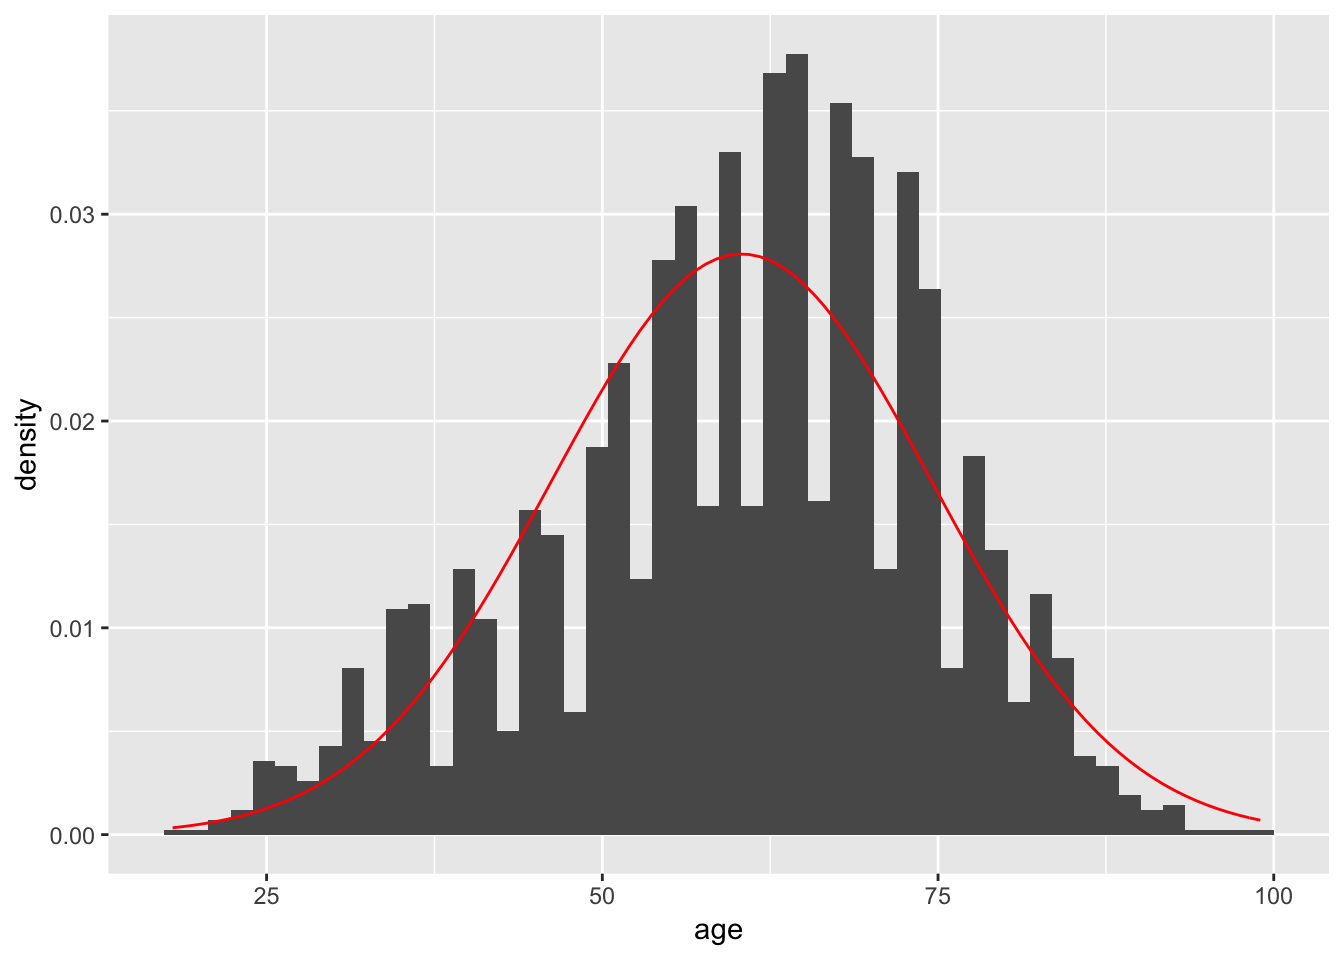
\includegraphics{lab3_files/figure-latex/3_norm-1.pdf}

Comparing the histogram plot to the normal distribution curve generated
may prove difficult. The \texttt{geom\_density()} function can draw a
line using density data for \emph{age} alongside the projected line of
what the normal distribution would appear like given the mean and
standard deviation. The two shapes can then be compared visually to
interpret whether the \emph{age} data can be approximated by the normal
distribution.

\begin{Shaded}
\begin{Highlighting}[]
\KeywordTok{ggplot}\NormalTok{(ds, }\KeywordTok{aes}\NormalTok{(age)) }\OperatorTok{+}
\StringTok{  }\KeywordTok{geom_histogram}\NormalTok{(}\KeywordTok{aes}\NormalTok{(}\DataTypeTok{x=}\NormalTok{age, }\DataTypeTok{y=}\NormalTok{..density..), }\DataTypeTok{bins=}\DecValTok{50}\NormalTok{) }\OperatorTok{+}
\StringTok{  }\KeywordTok{stat_function}\NormalTok{(}\DataTypeTok{fun=}\NormalTok{dnorm, }\DataTypeTok{args =} \KeywordTok{list}\NormalTok{(}\DataTypeTok{mean=}\KeywordTok{mean}\NormalTok{(ds}\OperatorTok{$}\NormalTok{age), }\DataTypeTok{sd=}\KeywordTok{sd}\NormalTok{(ds}\OperatorTok{$}\NormalTok{age)), }\DataTypeTok{color=}\StringTok{"red"}\NormalTok{) }\OperatorTok{+}
\StringTok{  }\KeywordTok{geom_density}\NormalTok{(}\DataTypeTok{color=}\StringTok{"blue"}\NormalTok{)}
\end{Highlighting}
\end{Shaded}

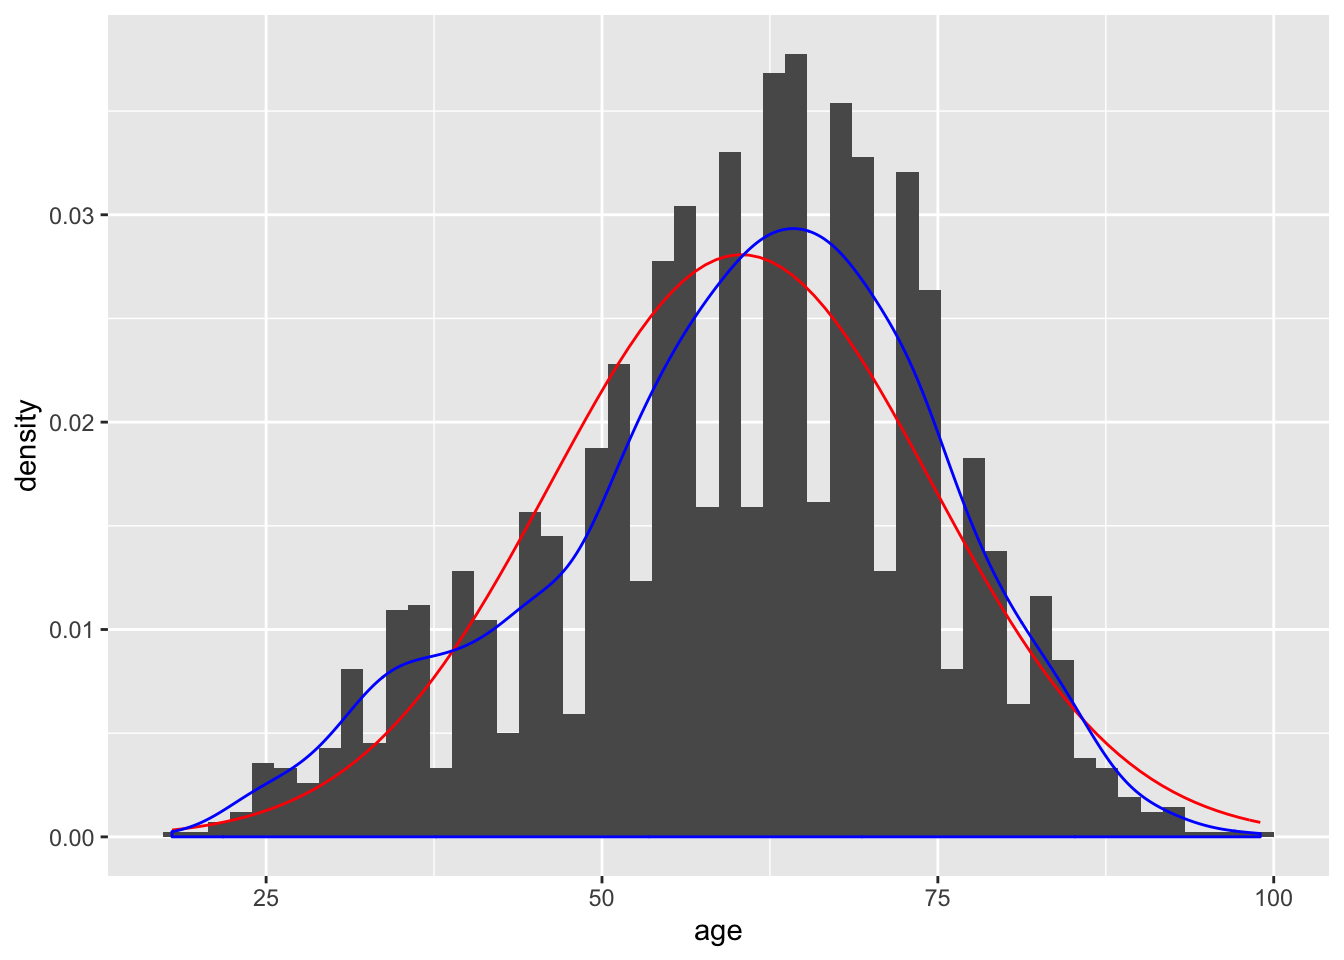
\includegraphics{lab3_files/figure-latex/3_norm2-1.pdf}

The culmination of the histogram, curve, and density line is improved
via the addition of limits and labels to the x-axis and y-axis, defining
a number of bins, and a chart title. Including fill and outline colors
for the histogram can also make it more readable:

\begin{Shaded}
\begin{Highlighting}[]
\KeywordTok{ggplot}\NormalTok{(ds, }\KeywordTok{aes}\NormalTok{(age)) }\OperatorTok{+}
\StringTok{  }\KeywordTok{geom_histogram}\NormalTok{(}\KeywordTok{aes}\NormalTok{(}\DataTypeTok{x=}\NormalTok{age, }\DataTypeTok{y=}\NormalTok{..density..), }\DataTypeTok{bins=}\DecValTok{50}\NormalTok{, }\DataTypeTok{fill=}\StringTok{"#d3d3d3"}\NormalTok{, }\DataTypeTok{color=}\StringTok{"black"}\NormalTok{) }\OperatorTok{+}
\StringTok{  }\KeywordTok{stat_function}\NormalTok{(}\DataTypeTok{fun=}\NormalTok{dnorm, }\DataTypeTok{args =} \KeywordTok{list}\NormalTok{(}\DataTypeTok{mean=}\KeywordTok{mean}\NormalTok{(ds}\OperatorTok{$}\NormalTok{age), }\DataTypeTok{sd=}\KeywordTok{sd}\NormalTok{(ds}\OperatorTok{$}\NormalTok{age)), }\DataTypeTok{color=}\StringTok{"red"}\NormalTok{) }\OperatorTok{+}
\StringTok{  }\KeywordTok{geom_density}\NormalTok{(}\DataTypeTok{color=}\StringTok{"blue"}\NormalTok{) }\OperatorTok{+}
\StringTok{  }\KeywordTok{ggtitle}\NormalTok{(}\StringTok{"Histogram of Age"}\NormalTok{) }\OperatorTok{+}
\StringTok{  }\KeywordTok{xlab}\NormalTok{(}\StringTok{"Age"}\NormalTok{) }\OperatorTok{+}
\StringTok{  }\KeywordTok{ylab}\NormalTok{(}\StringTok{"Density"}\NormalTok{) }\OperatorTok{+}
\StringTok{  }\KeywordTok{theme_bw}\NormalTok{() }\OperatorTok{+}
\StringTok{  }\KeywordTok{coord_cartesian}\NormalTok{(}\DataTypeTok{xlim=}\KeywordTok{c}\NormalTok{(}\DecValTok{15}\NormalTok{,}\DecValTok{95}\NormalTok{), }\DataTypeTok{ylim=}\KeywordTok{c}\NormalTok{(}\DecValTok{0}\NormalTok{,}\FloatTok{0.04}\NormalTok{))}
\end{Highlighting}
\end{Shaded}

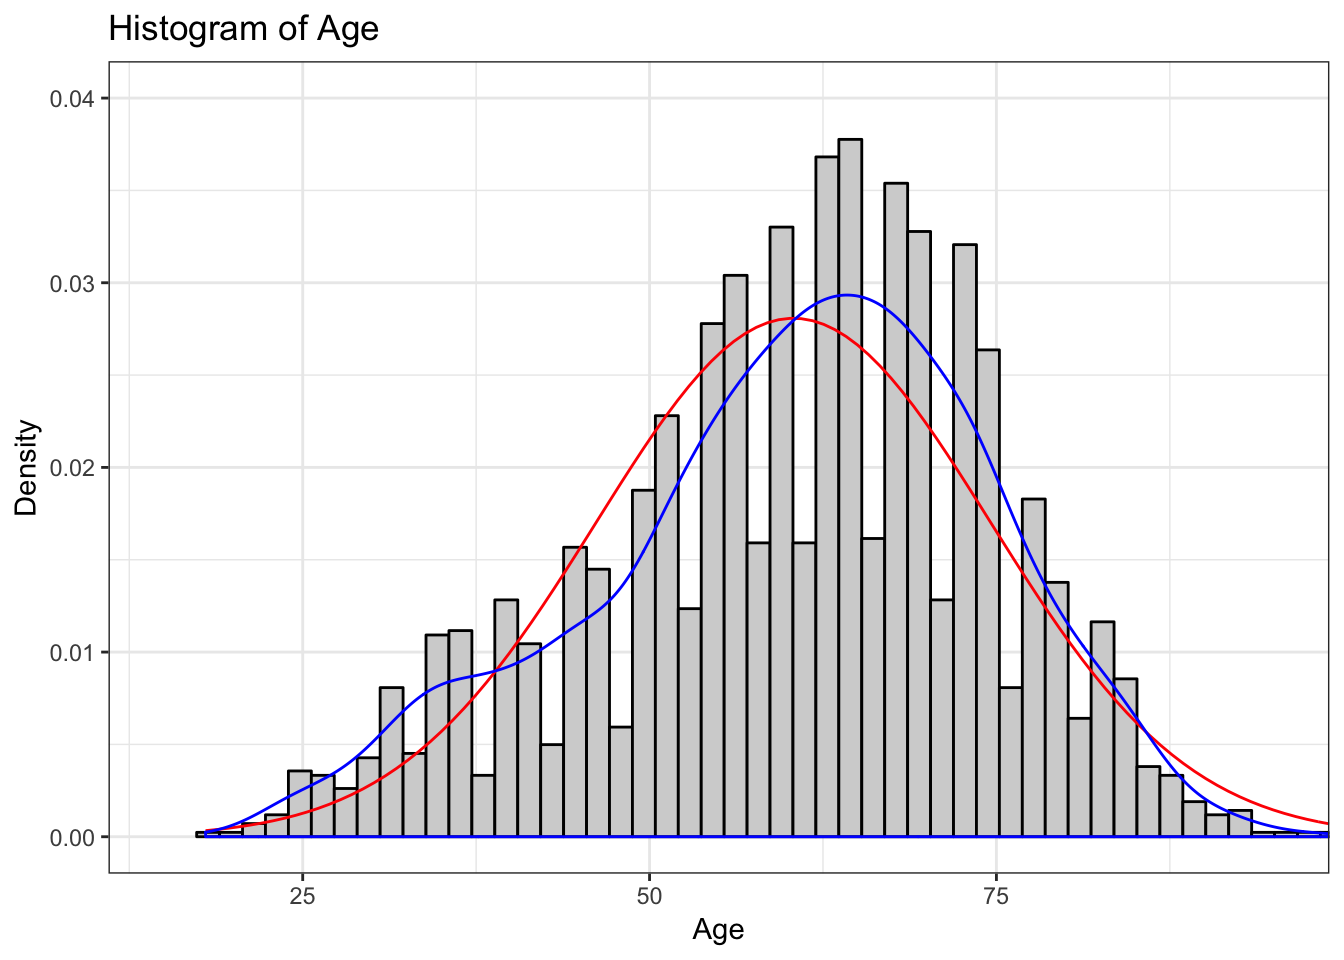
\includegraphics{lab3_files/figure-latex/3_norm3-1.pdf}

\subsection{Part II: Probability and
Distributions}\label{part-ii-probability-and-distributions}

R supports a number of distributions; however, for the purpose of these
labs we will focus primarily on the normal and binomial distributions.
View the \texttt{help(Distributions)} documentation to explore the
distributions supported by R.

help(Distributions)

The following R functions are applicable to the normal distribution:

\begin{enumerate}
\def\labelenumi{\arabic{enumi}.}
\tightlist
\item
  \texttt{dnorm()}
\item
  \texttt{pnorm()}
\item
  \texttt{qnorm()}
\item
  \texttt{rnorm()}
\end{enumerate}

The \texttt{dnorm()} function provides the height of a probability
distribution function at a given x value:
\texttt{dnorm(x,\ mean=\$\textbackslash{}mu\$,\ standard\ deviation=\$\textbackslash{}sigma\$)}.
\textbf{Note:} The value returned by the \texttt{dnorm()} function is
not the probability associated with the occurrence of the x value!

The default mean and standard deviation for the \texttt{dnorm()}
function is 0 and 1, respectively. The following example finds the
height of the probability distribution function at \(x=2\) with
\(\mu = 4\) and \(\sigma = 1.5\).

\begin{Shaded}
\begin{Highlighting}[]
\KeywordTok{dnorm}\NormalTok{(}\DecValTok{2}\NormalTok{, }\DataTypeTok{mean =} \DecValTok{4}\NormalTok{, }\DataTypeTok{sd=}\FloatTok{1.5}\NormalTok{)}
\end{Highlighting}
\end{Shaded}

\begin{verbatim}
## [1] 0.10934
\end{verbatim}

The \texttt{dnorm()} function used in conjunction with the \texttt{age}
variable from \texttt{ds} data set can find the height of the
probability distribution function. In the following example, the
\texttt{dnorm()} function will find the height of the probability
distribution function for 65. Similar to previous examples, an argument
exists to ignore NA and missing values.

\begin{Shaded}
\begin{Highlighting}[]
\KeywordTok{dnorm}\NormalTok{(}\DecValTok{65}\NormalTok{, }\DataTypeTok{mean=}\KeywordTok{mean}\NormalTok{(ds}\OperatorTok{$}\NormalTok{age, }\DataTypeTok{na.rm =}\NormalTok{ T), }\DataTypeTok{sd=}\KeywordTok{sd}\NormalTok{(ds}\OperatorTok{$}\NormalTok{age, }\DataTypeTok{na.rm=}\NormalTok{T))}
\end{Highlighting}
\end{Shaded}

\begin{verbatim}
## [1] 0.02662361
\end{verbatim}

The \texttt{dnorm()} returns the height of the probability distribution
function as 0.027. \textbf{Note:} This is a random value and, by itself,
is not meaningful. The \texttt{dnorm()} function returns the relative
likelihood, which can lead to determining a probability; however, to
understand this value further requires an explanation of calculus.

For continuous data, the probability of a single value is small (near
zero), so instead the approach should be to find the probability a value
occurs within a specified range. The probability associated to a value
occurring within a specified range is equal to the area of the
probability distribution function between the two points. In calculus
this is defined as finding the integral of the probability distribution
function.

\[\int_{-\x_1}^{x_2}{f_X(t)\,dx}\]

The above formula is the cumulative distribution function for two
points, \(x_1\) and \(x_2\). In this case, \(x_1\) is defined as the
lower bound and \(x_2\) is defined as the upper bound.

R includes the calculus function \texttt{integrate.xy()} to return the
probability.

\begin{Shaded}
\begin{Highlighting}[]
\KeywordTok{integrate.xy}\NormalTok{(}\KeywordTok{density}\NormalTok{(ds}\OperatorTok{$}\NormalTok{age)}\OperatorTok{$}\NormalTok{x,}\KeywordTok{density}\NormalTok{(ds}\OperatorTok{$}\NormalTok{age)}\OperatorTok{$}\NormalTok{y,}\DecValTok{65}\NormalTok{,}\DecValTok{66}\NormalTok{)}
\end{Highlighting}
\end{Shaded}

\begin{verbatim}
## [1] 0.02917993
\end{verbatim}

The probability associated to an age between 65 and 66 in the
\texttt{age} variable is .029 (\(\approx\) 3\% chance).

Similarly, the \texttt{pnorm()} function calculates probabilities
associated to a given x value. The default for the \texttt{pnorm()}
function is the cumulative distribution function with a lower bound of
\(-\infty\) and an upper bound of x.

The following example calculates the probability associated to an age
value between \(-\infty\) and 5, given \(\mu = 6\) and \(\sigma = 6\).

\begin{Shaded}
\begin{Highlighting}[]
\KeywordTok{pnorm}\NormalTok{(}\DecValTok{5}\NormalTok{, }\DataTypeTok{mean =} \DecValTok{6}\NormalTok{, }\DataTypeTok{sd =} \DecValTok{2}\NormalTok{)}
\end{Highlighting}
\end{Shaded}

\begin{verbatim}
## [1] 0.3085375
\end{verbatim}

The \texttt{pnorm()} calculates the probability of observing a value
between \(-\infty\) and 5 as 0.31. The following example uses the
\texttt{pnorm()} function with the \texttt{ds} data set to find the
probability that a respondent is 65 or less years old.

\begin{Shaded}
\begin{Highlighting}[]
\KeywordTok{pnorm}\NormalTok{(}\DecValTok{65}\NormalTok{, }\DataTypeTok{mean=}\KeywordTok{mean}\NormalTok{(ds}\OperatorTok{$}\NormalTok{age, }\DataTypeTok{na.rm=}\NormalTok{T), }\DataTypeTok{sd=}\KeywordTok{sd}\NormalTok{(ds}\OperatorTok{$}\NormalTok{age, }\DataTypeTok{na.rm =}\NormalTok{ T))}
\end{Highlighting}
\end{Shaded}

\begin{verbatim}
## [1] 0.6277983
\end{verbatim}

To calculate the probability associated to an age of 65 or greater, the
\texttt{lower.tail\ =\ FALSE} argument will look at the upper tail
(right side of the probability distribution function). This is equal to
the difference between 1 and the lower tail probability previously
calculated.

\begin{Shaded}
\begin{Highlighting}[]
\KeywordTok{pnorm}\NormalTok{(}\DecValTok{65}\NormalTok{, }\DataTypeTok{mean=}\KeywordTok{mean}\NormalTok{(ds}\OperatorTok{$}\NormalTok{age, }\DataTypeTok{na.rm =}\NormalTok{ T), }\DataTypeTok{sd=}\KeywordTok{sd}\NormalTok{(ds}\OperatorTok{$}\NormalTok{age, }\DataTypeTok{na.rm =}\NormalTok{ T), }\DataTypeTok{lower.tail =} \OtherTok{FALSE}\NormalTok{)}
\end{Highlighting}
\end{Shaded}

\begin{verbatim}
## [1] 0.3722017
\end{verbatim}

The \texttt{qnorm()} function is the inverse function of the
\texttt{pnorm()} function. Given a probability, mean, and standard
deviation, the \texttt{qnorm()} function will return an x value from the
probability distribution function. The following example finds the upper
bound x value of the probability distribution function associated to the
probability, or area under the curve, of 0.3 given \(\mu = 5\) and
\(\sigma = 1\).

\begin{Shaded}
\begin{Highlighting}[]
\KeywordTok{qnorm}\NormalTok{(.}\DecValTok{3}\NormalTok{, }\DataTypeTok{mean=}\DecValTok{5}\NormalTok{, }\DataTypeTok{sd=}\DecValTok{1}\NormalTok{)}
\end{Highlighting}
\end{Shaded}

\begin{verbatim}
## [1] 4.475599
\end{verbatim}

The following calculates the upper bound age from the \texttt{age}
variable in the \texttt{ds} data set to demonstrate further associated
to a 40\% probability. That is, the \texttt{qnorm()} function calculates
the age that 40\% of respondents are equal or less to.

\begin{Shaded}
\begin{Highlighting}[]
\KeywordTok{qnorm}\NormalTok{(.}\DecValTok{4}\NormalTok{, }\DataTypeTok{mean=}\KeywordTok{mean}\NormalTok{(ds}\OperatorTok{$}\NormalTok{age, }\DataTypeTok{na.rm =}\NormalTok{ T), }\DataTypeTok{sd=}\KeywordTok{sd}\NormalTok{(ds}\OperatorTok{$}\NormalTok{age, }\DataTypeTok{na.rm =}\NormalTok{ T))}
\end{Highlighting}
\end{Shaded}

\begin{verbatim}
## [1] 56.7677
\end{verbatim}

Lastly, the \texttt{rnorm()} function will generate random values that
follow a normal distribution given a number of points (n), provided
\(\mu\), and \(\sigma\). The following example calculates 200 random
values given \(\mu = 6\) and \(\sigma = 2\). The random values are
stored to the \texttt{rvalues} object.

\begin{Shaded}
\begin{Highlighting}[]
\NormalTok{rvalues <-}\StringTok{ }\KeywordTok{rnorm}\NormalTok{(}\DecValTok{200}\NormalTok{, }\DataTypeTok{mean=}\DecValTok{6}\NormalTok{, }\DataTypeTok{sd=}\DecValTok{2}\NormalTok{)}
\KeywordTok{ggplot}\NormalTok{() }\OperatorTok{+}
\StringTok{  }\KeywordTok{geom_histogram}\NormalTok{(}\KeywordTok{aes}\NormalTok{(rvalues), }\DataTypeTok{bins=}\DecValTok{14}\NormalTok{)}
\end{Highlighting}
\end{Shaded}

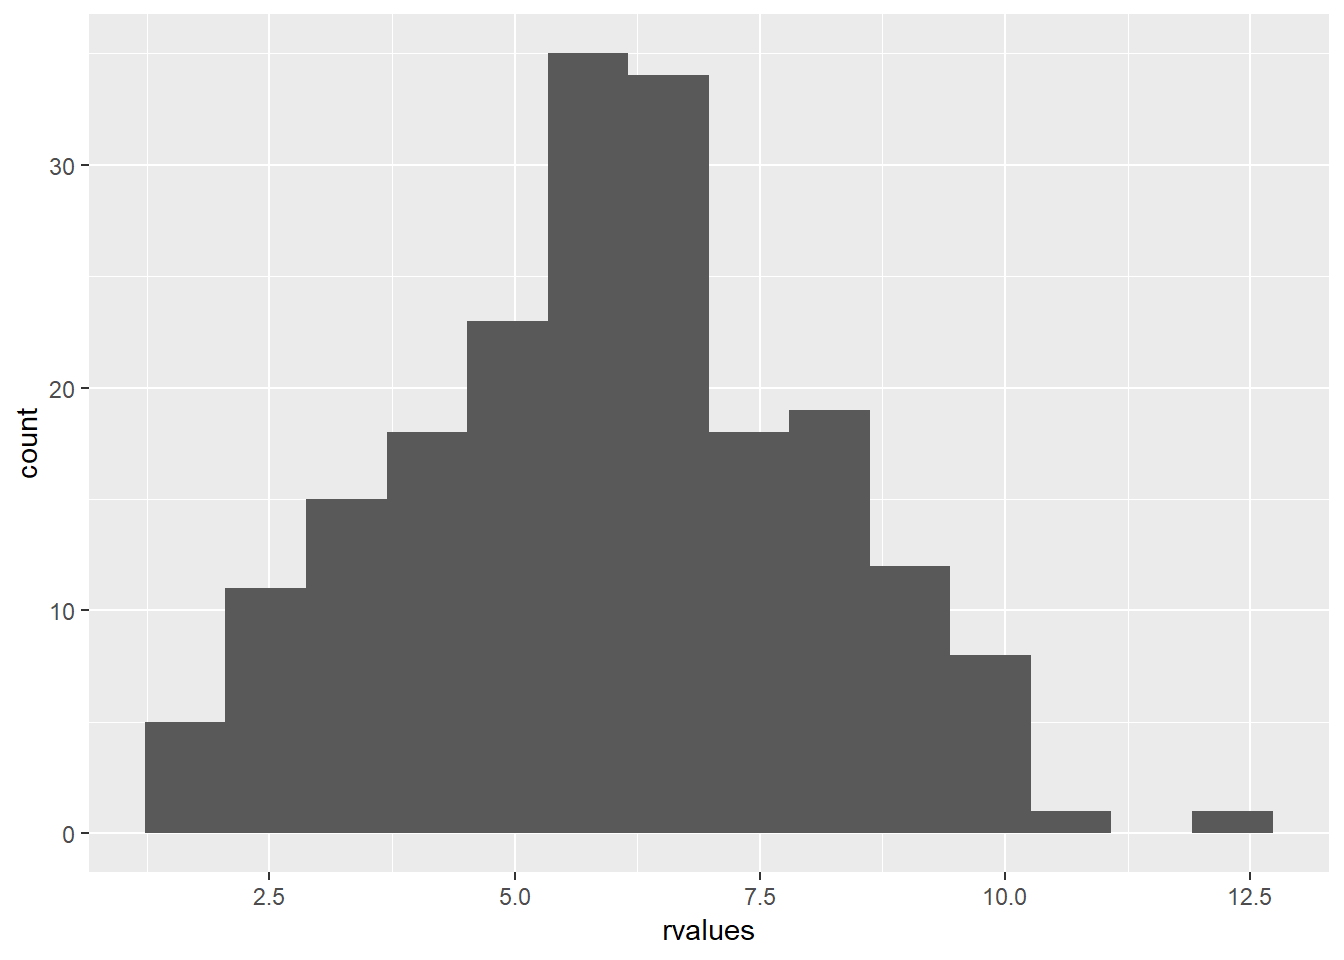
\includegraphics{lab3_files/figure-latex/3_rnorm-1.pdf}

\textbf{Note:} The discussed functions are relevant to the normal
distribution functions provided by R. R includes similar functions for
other distributions, with equivalent functionality.

\subsection{Part III: Visualizing
Normality}\label{part-iii-visualizing-normality}

Thus far the normal distribution has been discussed without
visualization. When graphed, data that follow a normal distribution
resemble a bell shaped curve. To demonstrate, the following code employs
the \texttt{rnorm()} function to generate 1000 random values with
\(\mu = 100\) and \(\sigma = 20\), and assigns the values to an object
named \texttt{random}.

\begin{Shaded}
\begin{Highlighting}[]
\NormalTok{random <-}\StringTok{ }\KeywordTok{rnorm}\NormalTok{(}\DecValTok{1000}\NormalTok{, }\DataTypeTok{mean =} \DecValTok{100}\NormalTok{, }\DataTypeTok{sd =} \DecValTok{20}\NormalTok{)}
\end{Highlighting}
\end{Shaded}

Inspecting a density histogram of the \texttt{random} object yields a
bell shaped curve.

\begin{Shaded}
\begin{Highlighting}[]
\KeywordTok{ggplot}\NormalTok{() }\OperatorTok{+}
\StringTok{  }\KeywordTok{geom_histogram}\NormalTok{(}\KeywordTok{aes}\NormalTok{(random, ..density..), }\DataTypeTok{fill=}\StringTok{"white"}\NormalTok{, }\DataTypeTok{color=}\StringTok{"black"}\NormalTok{)}
\end{Highlighting}
\end{Shaded}

\begin{verbatim}
## `stat_bin()` using `bins = 30`. Pick better value with `binwidth`.
\end{verbatim}

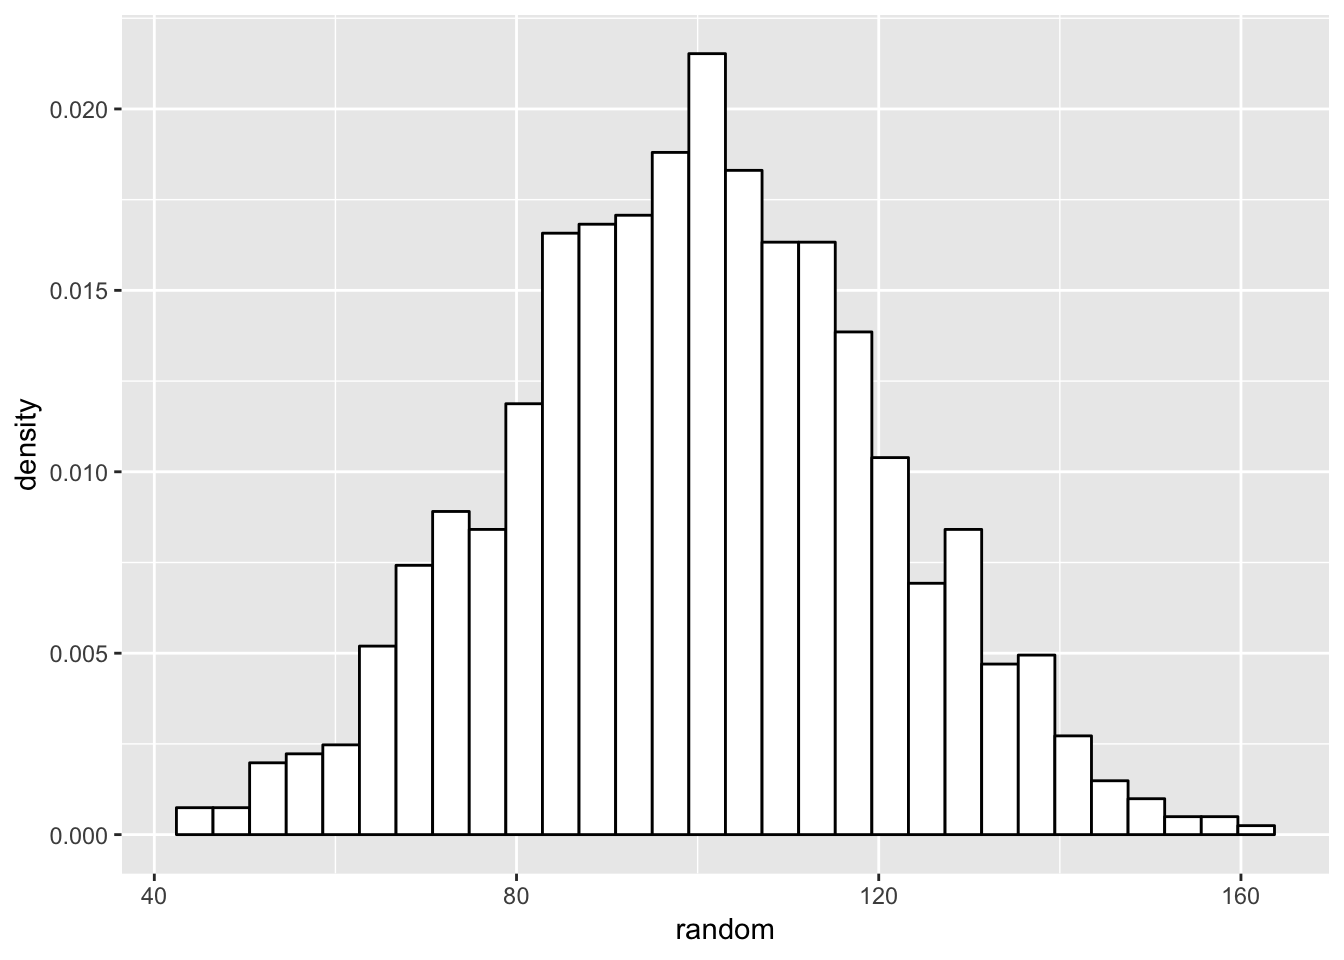
\includegraphics{lab3_files/figure-latex/3_three2-1.pdf}

Let's start figuring out how to check if our data is normally
distributed. There are many packages than will generate a density curve
of your data and a projected normal distribution for comparison, but
building all of the visualizations in ggplot provides both an intuitive
and informative method of doing so. Start by creating a density plot of
the randomly generated data.

Let's start figuring out how to check if our data is normally
distributed. At the beginning of this lab we should have installed and
loaded the package ``sm''. We use the \texttt{sm.density()} function to
visualize data and to project what should be the normal distribution of
the data, given the mean and standard deviation of the data. Let's start
with our randomly generated data. We include the \texttt{model="Normal"}
argument at the end of the function, so that \texttt{sm.density} knows
to use the normal distribution.

\begin{Shaded}
\begin{Highlighting}[]
\KeywordTok{ggplot}\NormalTok{() }\OperatorTok{+}
\StringTok{  }\KeywordTok{geom_density}\NormalTok{(}\KeywordTok{aes}\NormalTok{(random))}
\end{Highlighting}
\end{Shaded}

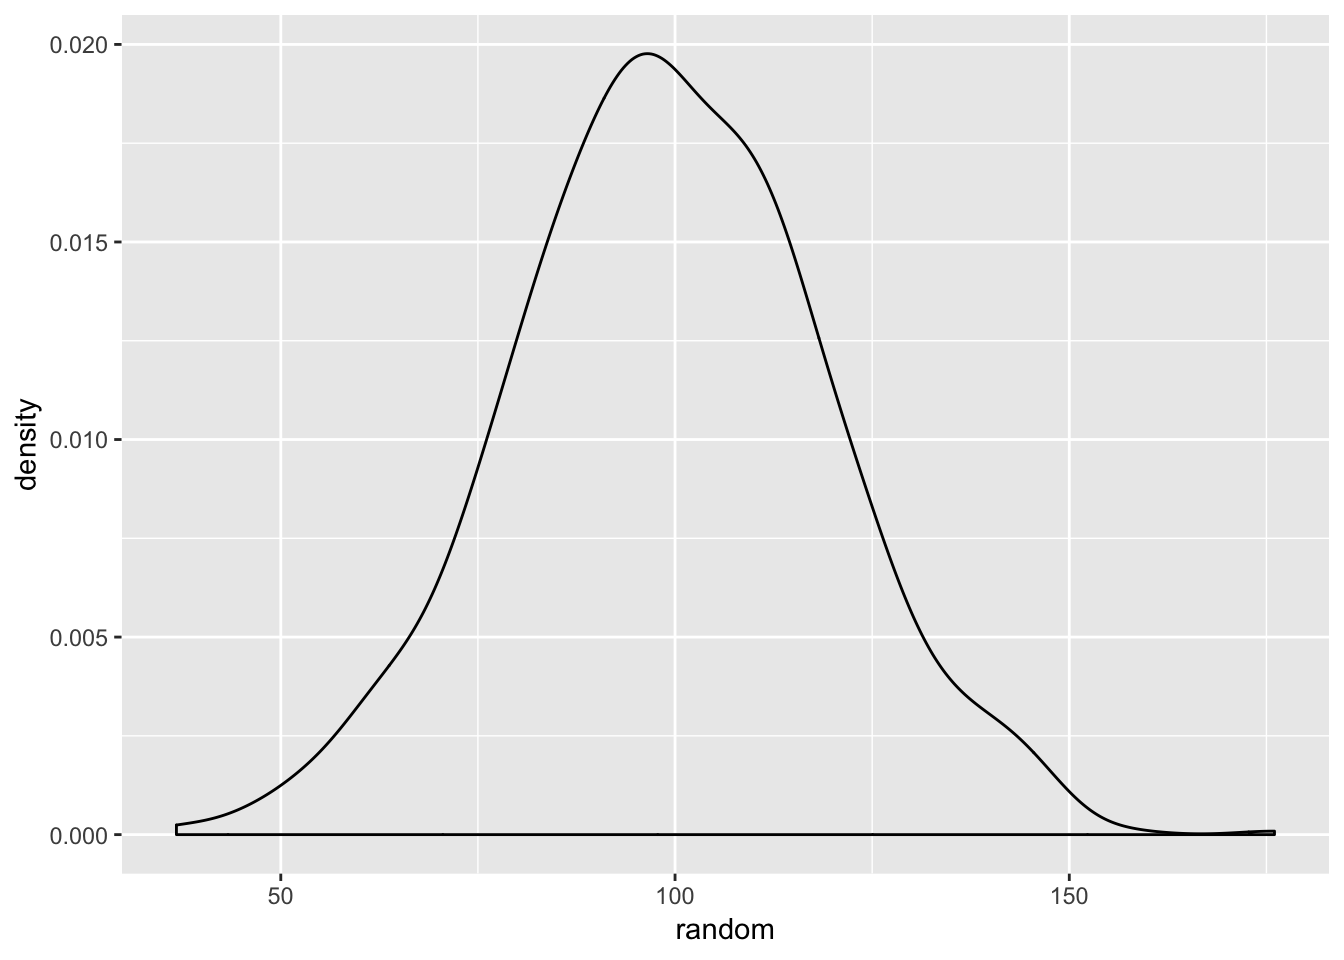
\includegraphics{lab3_files/figure-latex/3_three4-1.pdf}

Given the \texttt{random} values consists of values generated by the
\texttt{rnorm()} function, this distrubtion resembling the normal
distribution is unsurprising.

The following code generates a density line for the \texttt{age}
variable from the \texttt{ds} data set and a projected normal
distribution given the mean and standaard deviation of the variable.
Indicating \texttt{alpha=.5} will make the line slightly transparent.

\begin{Shaded}
\begin{Highlighting}[]
\KeywordTok{ggplot}\NormalTok{(ds, }\KeywordTok{aes}\NormalTok{(age)) }\OperatorTok{+}
\StringTok{  }\KeywordTok{geom_density}\NormalTok{(}\KeywordTok{aes}\NormalTok{(ds}\OperatorTok{$}\NormalTok{age)) }\OperatorTok{+}
\StringTok{  }\KeywordTok{stat_function}\NormalTok{(}\DataTypeTok{fun=}\NormalTok{dnorm, }\DataTypeTok{args=}\KeywordTok{list}\NormalTok{(}\DataTypeTok{mean=}\KeywordTok{mean}\NormalTok{(ds}\OperatorTok{$}\NormalTok{age), }\DataTypeTok{sd=}\KeywordTok{sd}\NormalTok{(ds}\OperatorTok{$}\NormalTok{age)), }\DataTypeTok{color=}\StringTok{"red"}\NormalTok{, }\DataTypeTok{size=}\DecValTok{2}\NormalTok{, }\DataTypeTok{alpha=}\NormalTok{.}\DecValTok{5}\NormalTok{)}
\end{Highlighting}
\end{Shaded}

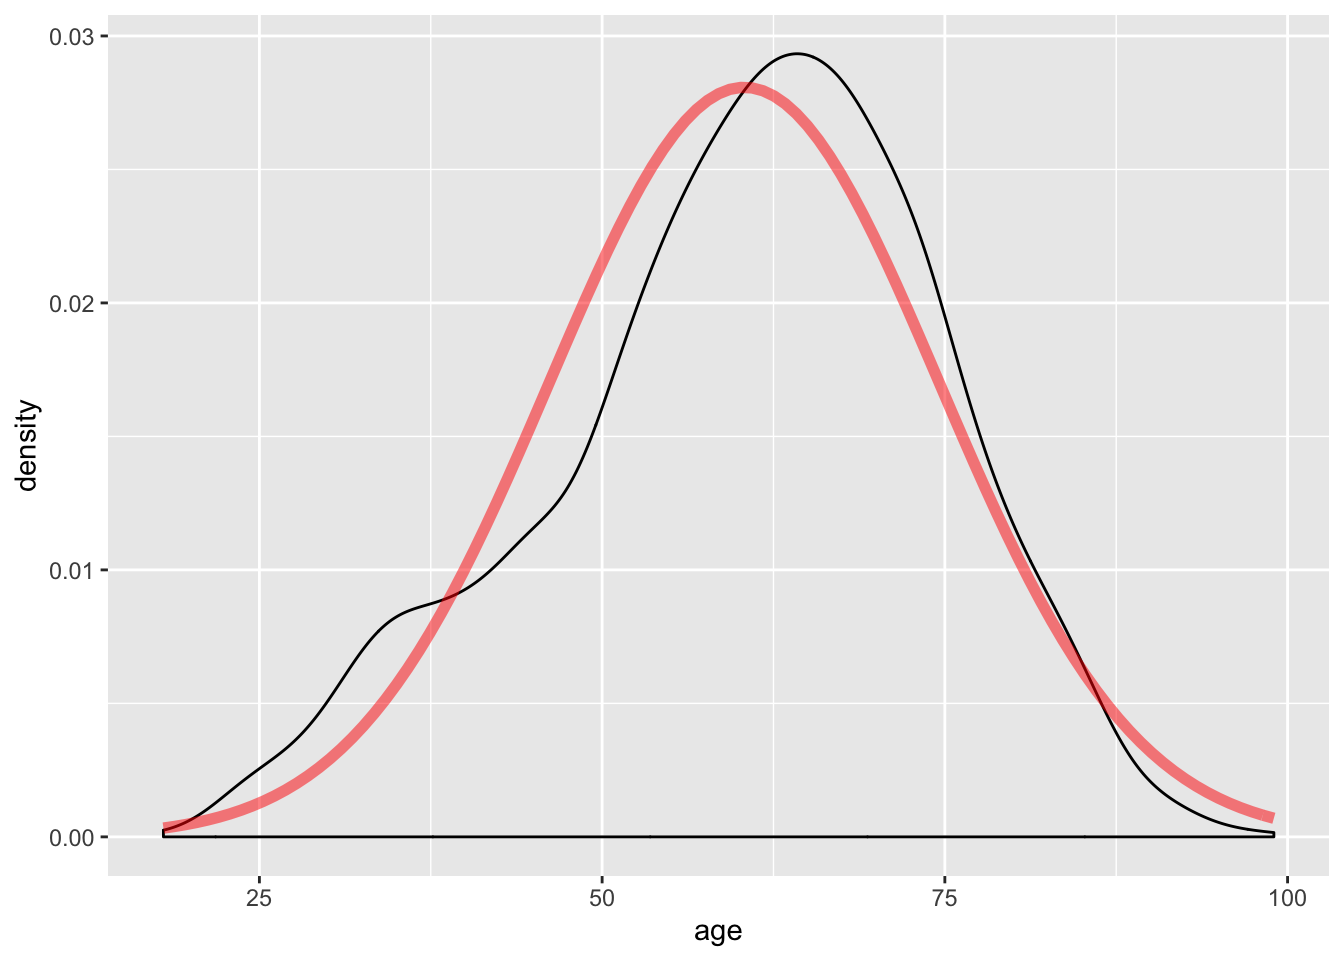
\includegraphics{lab3_files/figure-latex/3_three5-1.pdf}

The shape of the density line closely resembles a normal distribution;
however, note the slight skew.

Another method to view whether data follows a normal distribution is to
view the QQ plot, available via the \texttt{qqPlot()} function.

A QQ plot visualizes data based on the quantiles of the provided
variable against the quantiles that would exist if the data were
normally distributed. Data that follows the normal distribution should
be in a line with a set slope. Including \texttt{stat\_qq()} generates a
QQ plot. The following example generates a QQ plot of the \texttt{age}
variable.

\begin{Shaded}
\begin{Highlighting}[]
\KeywordTok{ggplot}\NormalTok{(ds, }\KeywordTok{aes}\NormalTok{(}\DataTypeTok{sample=}\NormalTok{age)) }\OperatorTok{+}
\StringTok{  }\KeywordTok{stat_qq}\NormalTok{()}
\end{Highlighting}
\end{Shaded}

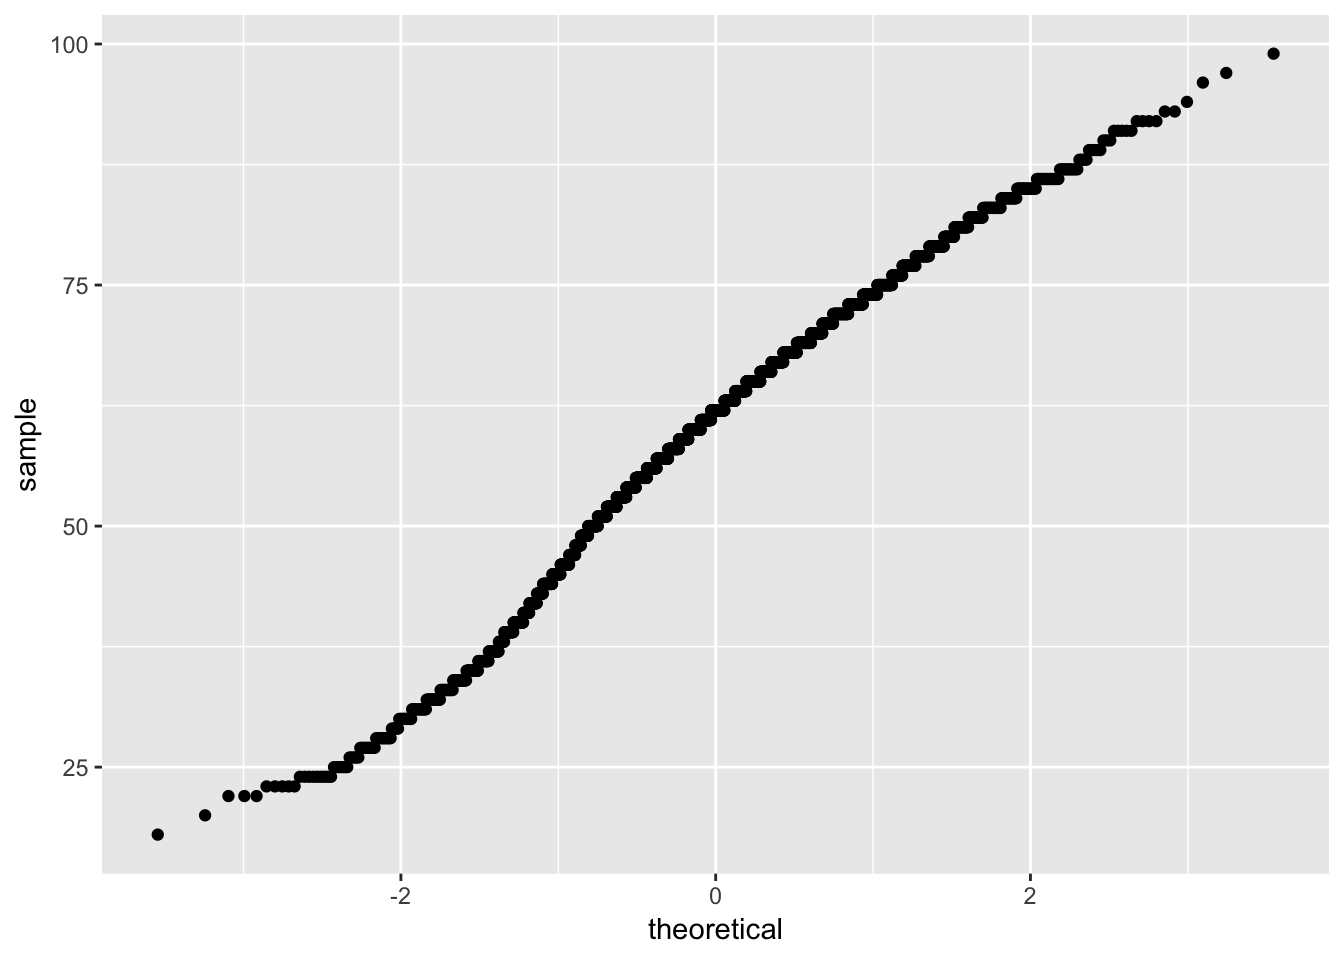
\includegraphics{lab3_files/figure-latex/3_three6-1.pdf}

To further inspect the normality, a diagonal line can be generated that
will visualize what the slope of the data should be if it were normally
distributed. To include such a line, use \texttt{geom\_abline()}. The
slope and intercept of the line must also be calculated. Doing so
requires a small amount of basic linear algebra. Find the first and
third quantiles of the \texttt{age} variable and set it to an object
named \texttt{y}, then find the theoretical first and third quantiles
for normally-distributed data and set it to \texttt{x}. Calculate the
slope by taking the diference in \texttt{y} over the difference in
\texttt{x} and set that to an object named \texttt{slope}. Then solve
for the intercept and it it to an object named \texttt{intercept}.

\begin{Shaded}
\begin{Highlighting}[]
\NormalTok{y     <-}\StringTok{ }\KeywordTok{quantile}\NormalTok{(ds}\OperatorTok{$}\NormalTok{age, }\KeywordTok{c}\NormalTok{(}\FloatTok{0.25}\NormalTok{, }\FloatTok{0.75}\NormalTok{)) }\CommentTok{# Find the 1st and 3rd quantiles}
\NormalTok{x     <-}\StringTok{ }\KeywordTok{qnorm}\NormalTok{( }\KeywordTok{c}\NormalTok{(}\FloatTok{0.25}\NormalTok{, }\FloatTok{0.75}\NormalTok{))           }\CommentTok{# Find the matching normal values on the x-axis}
\NormalTok{slope <-}\StringTok{ }\KeywordTok{diff}\NormalTok{(y) }\OperatorTok{/}\StringTok{ }\KeywordTok{diff}\NormalTok{(x)               }\CommentTok{# Compute the line slope}
\NormalTok{int   <-}\StringTok{ }\NormalTok{y[}\DecValTok{1}\NormalTok{] }\OperatorTok{-}\StringTok{ }\NormalTok{slope }\OperatorTok{*}\StringTok{ }\NormalTok{x[}\DecValTok{1}\NormalTok{]             }\CommentTok{# Compute the line intercept}

\KeywordTok{ggplot}\NormalTok{(ds, }\KeywordTok{aes}\NormalTok{(}\DataTypeTok{sample =}\NormalTok{ age)) }\OperatorTok{+}
\StringTok{  }\KeywordTok{stat_qq}\NormalTok{() }\OperatorTok{+}\StringTok{ }
\StringTok{  }\KeywordTok{geom_abline}\NormalTok{(}\DataTypeTok{intercept =}\NormalTok{ int, }\DataTypeTok{slope =}\NormalTok{ slope, }\DataTypeTok{color =} \StringTok{"blue"}\NormalTok{, }\DataTypeTok{size =} \DecValTok{2}\NormalTok{, }\DataTypeTok{alpha =} \FloatTok{0.5}\NormalTok{ )}
\end{Highlighting}
\end{Shaded}

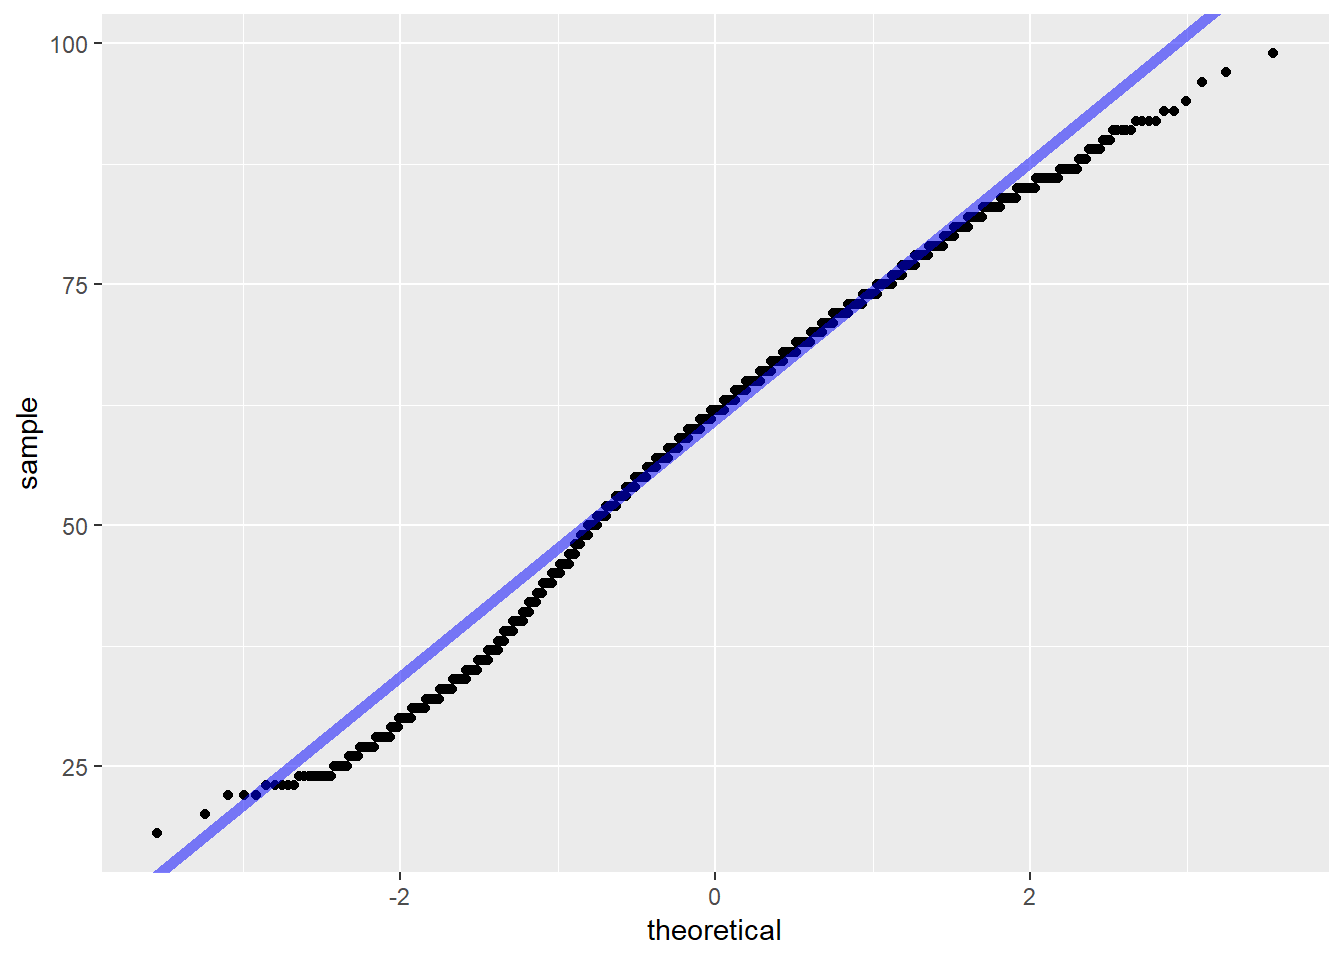
\includegraphics{lab3_files/figure-latex/3_three7-1.pdf}

In the graphic above, the solid blue line exhibits where data should
fall if it follows a normal distribution, and the blue dash lines
represent confidence intervals. The individual circles represent data
points from the variable. If the data points is within the intervals,
then the data likely follows a normal distribution. The interpretation
of this QQ plot yields that the data likely follows a normal
distribution, as expected given the data was generated via the
\texttt{rnorm()} function.

The QQ plot confirms the sm.density() plot: the \texttt{age} variable
closely follows a normal distribution. Note that some values are outside
the confidence interval. These are the points associated to the skew
previously observed.

Another last method to inspect whether data follows a normal
distribution is the box plot. Box plots provides quartiles and the
median, and returns individual unique values at the edges of our data.
The following code generates a box plot of the \texttt{age} variable.

\begin{Shaded}
\begin{Highlighting}[]
\KeywordTok{ggplot}\NormalTok{(ds, }\KeywordTok{aes}\NormalTok{(}\DataTypeTok{x=}\StringTok{""}\NormalTok{, }\DataTypeTok{y=}\NormalTok{age)) }\OperatorTok{+}
\StringTok{  }\KeywordTok{geom_boxplot}\NormalTok{()}
\end{Highlighting}
\end{Shaded}

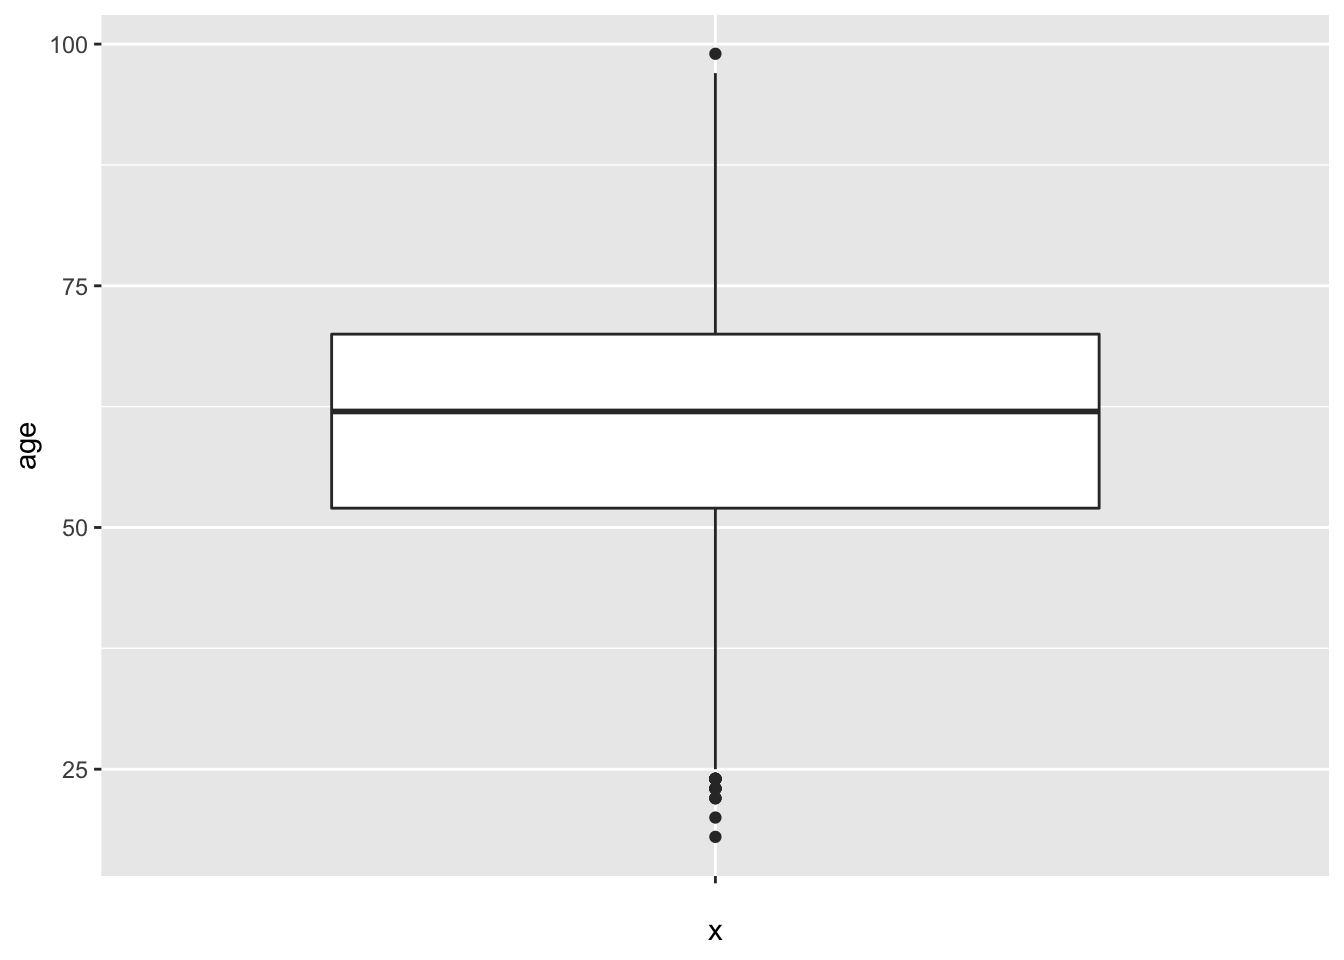
\includegraphics{lab3_files/figure-latex/3_three8-1.pdf}

Note the middle line is the middle quartile, or the median. The distance
between the median line and the line below it represents the second
quartile. The distance from the bottom of the second quartile line to
the very bottom line, or ``whisker'' is the first quartile. Above the
median, the distance between the median line and the next line above it
is the third quartile, and the area above that, and below the top
whisker, is the fourth quartile. Notice that for the box plot of our
randomly generated data, the distance between quartiles is relatively
even.

The distance between quartiles is relatively even; however, note the
difference to the previously generated box plot from the
\texttt{rnorm()} data.

\subsection{Part IV: Z-Scores}\label{part-iv-z-scores}

Standardizing, or scaling, data provides conveniences in discussing
data. For instance, discussing how many standard deviations a particular
value occurs from the mean is more meaningful than purely the distance.
Scaling data in terms of z-scores provides the number of standard
deviations a value is from the mean.

The following example employs the \texttt{scale()} function to calculate
z-score for each data point and assigns them to a newly created
\texttt{z.age} variable in the \texttt{ds} data set. To do this, use the
\texttt{mutate()} verb, which is a tidyverse function that creates new
variables or modifies existing variables:

\begin{Shaded}
\begin{Highlighting}[]
\NormalTok{ds }\OperatorTok
\StringTok{  }\KeywordTok{mutate}\NormalTok{(}\DataTypeTok{z.age =} \KeywordTok{scale}\NormalTok{(age)) ->}\StringTok{ }\NormalTok{ds}
\end{Highlighting}
\end{Shaded}

Using a filter approach, the following example finds the z-score
associated to women younger than 19 years old. First filter the data
with the preferred stipulations, then use the \texttt{select()} verb
from the \texttt{dplyr()} package (part of the tidyverse!) to view the
results. All of this is connected using the pipe function,
\%\textgreater{}\%.

\begin{Shaded}
\begin{Highlighting}[]
\NormalTok{ds }\OperatorTok\StringTok{ }
\StringTok{  }\KeywordTok{filter}\NormalTok{(f.gender }\OperatorTok{==}\StringTok{ "Women"} \OperatorTok{&}\StringTok{ }\NormalTok{age }\OperatorTok{<}\StringTok{ }\DecValTok{19}\NormalTok{) }\OperatorTok
\StringTok{  }\NormalTok{dplyr}\OperatorTok{::}\KeywordTok{select}\NormalTok{(f.gender, age, z.age)}
\end{Highlighting}
\end{Shaded}

\begin{verbatim}
## # A tibble: 1 x 3
##   f.gender   age z.age
##   <chr>    <int> <dbl>
## 1 Women       18 -2.98
\end{verbatim}

The result shows that, within the \texttt{ds} data set, there is one
respondent that identified as a woman under 19 years old. The z-score
for this respondent is -2.98, which is interpreted as this respondent's
age is 2.98 standard deviations below the mean.

Given a z-score, the mean age of respondents is assumed as much higher
than the 18 year old woman. The difference between the mean age of
respondents and the woman is the product of the z-score and standard
deviation. The following calculates the standard deviation of the
\texttt{age} variable.

\begin{Shaded}
\begin{Highlighting}[]
\KeywordTok{sd}\NormalTok{(ds}\OperatorTok{$}\NormalTok{age, }\DataTypeTok{na.rm =} \OtherTok{TRUE}\NormalTok{)}
\end{Highlighting}
\end{Shaded}

\begin{verbatim}
## [1] 14.20894
\end{verbatim}

The \texttt{sd()} function returns the standard deviation of data. The
product of the \texttt{sd()} function and calculated z-score, is the
difference between the 18 year old woman and mean age of respondents.

\begin{Shaded}
\begin{Highlighting}[]
\FloatTok{2.981748}\OperatorTok{*}\KeywordTok{sd}\NormalTok{(ds}\OperatorTok{$}\NormalTok{age, }\DataTypeTok{na.rm =} \OtherTok{TRUE}\NormalTok{)}
\end{Highlighting}
\end{Shaded}

\begin{verbatim}
## [1] 42.36748
\end{verbatim}

The difference between the 18 year old woman and mean age of respondents
is \(\approx\) 43.38 years.


\end{document}
